
%%%%%%%%%%%%%%%%%%%%%%%%%%%%%%%%%%%%%%%%%%%%%%%%%%%
\section{Platform}
\label{sec:components}
%%%%%%%%%%%%%%%%%%%%%%%%%%%%%%%%%%%%%%%%%%%%%%%%%%%




\begin{figure}
 \centering
  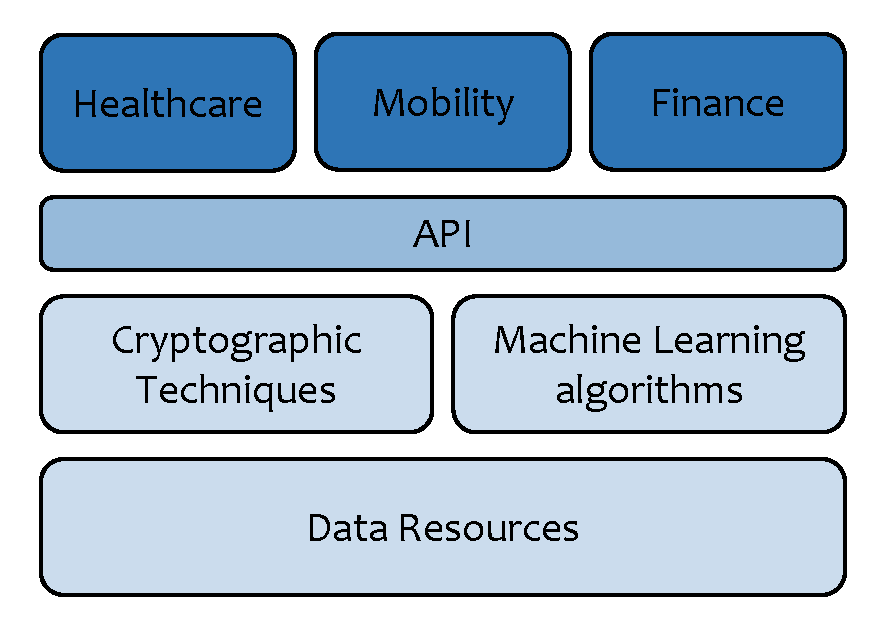
\includegraphics[width=0.5\textwidth]{images/conceptual_view_of_the_platform.pdf}
  \caption{Conceptual view of the platform.}
  \label{fig:ConceptView}
\end{figure}

In Figure \ref{fig:ConceptView} we present the conceptual view of our platform. 
The \emph{data resources} represent the datasets that are used in the classification process. 
The data processing itself is done using the combination of ML algorithms and cryptographic techniques for performing privacy-preserving computations. 
The Application Programming Interface (API) layer abstracts details and provides the operations of the platform itself, which allow a simplified building of applications and data visualizations.
The use-cases describe the various subjects that can be addressed using this platform, and allow us to place it in real-world scenarios that have high impact and demand in Big Data operations. More use-cases are possible beyond Healthcare, Mobility and Finance, as the platform is designed for general use.




% Joining the algorithms and techniques described in the previous sections, we propose now the creation of a platform that would allow developers to create, implement, and expand the existing components. 


% \begin{itemize}
%   \item What \ac{ml} algorithm to use.
%   \item What privacy-preserving technique to use.
%   \item The dataset to process.
%   \item Inspect the resulting data.
% \end{itemize}



% Finally, we now present how \acs{bard} could be implemented in a business scenario. The users, in this case, the companies that profit from using \acs{bard} to do knowledge learning, provide the dataset to train the model or select an existing model already trained with publicly available data, and provide the sample to be evaluated. A team of developers, that could be outsourced or part of the company, maintain the toolkit and develop new functionalities (new \ac{ml} algorithms, new privacy-preserving techniques, etc.). A central repository, that contains \ac{ml} models trained \textit{a priori} for different types of data context (healthcare, income, etc.). In Figure , we present a context diagram for \acs{bard}. 
